\section{TOR (The Onion Router)}
TOR aka. ‘\textit{The Onion Router}’ is described on the project
website\footnote{https://www.torproject.org/ } like this; “\textit{Tor is
free software and an open network that helps you defend against traffic
analysis, a form of network surveillance that threatens personal freedom
and privacy, confidential business activities and relationships, and
state security.}”
\\
\\
\noindent
TOR, in essence, hides your real IP address and instead provides you with
a so called \textit{.onion} address that should be extremely difficult to
de-anonymise for any attacker. A normal IP might look like this: 123.45.67.8
and an \textit{.onion} address might look like this:
\textit{fpzcf23ifxpiucjm.onion}. When you broadcast your normal IP address
it will be possible for an adversary to identify you through your internet
service provider that will hold all the data on all connections. If you
broadcast a .onion address only this is not possible and any traffic can
only be traced back to another hidden node on the TOR network. Spectrecoin
has TOR ‘\textit{built-in}’ and running as a process and when you start the
software you will connect to the TOR network with an \textit{.onion} address
and you will not broadcast your real IP address through the Spectrecoin
software for as long as you use the software. The Spectrecoin network will
reject all non-TOR connections.
\\
\\
\noindent
We are aware of ongoing discussions about TOR vs. I2P\footnote{https://geti2p.net/en/}
vs. Monero’s Kovri project that is currently under development. You can
read up on this, but it is clear that both may have both advantages and
disadvantages. TOR is in wider use and will have more development effort
behind. We are also aware of technology such as Dandelion and we will keep
an eye on developments in this area of network security and we are
considering this.
\\
\\
\noindent
If you want yet another layer of network security, you can also use a VPN
service with TOR so explore this if you feel that you need this level of
security.


\subsection{OBFS4}
OBFS4 is what is known as a TOR ‘\textit{pluggable Transport}’ and is a
means to hide the fact that you are connecting using TOR. A range of
countries including China and Iran for example are using technology to
block TOR traffic and we have implemented this to try and circumvent any
such censorship. It’s also useful to bear in mind that some countries might
view a TOR user with suspicion although it’s not blocked. When you go to
the download page for Spectrecoin look for the OBFS4 versions of the
software.



\begin{figure}[h]
	\centering
	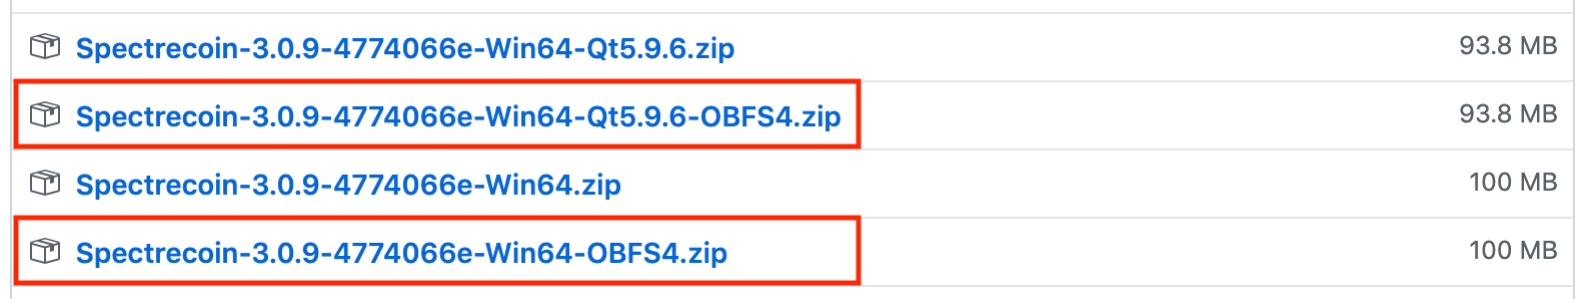
\includegraphics[width=\textwidth]{OBFS4-Walletversions.png}
	\caption{Spectrecoin wallet version with includet OBFS4}
\end{figure}

\newpage
\noindent
It’s difficult to say with 100\% certainty which countries block TOR but
you can find more information on 
this\footnote{https://metrics.torproject.org/userstats-bridge-table.html}
topic on the TOR project website, that will show you the top 10 countries
where TOR bridges are used. This\footnote{https://grobox.de/tor/} website
may also be of interest and for further information on TOR bridges and
transports you can find a lot of information
here\footnote{https://2019.www.torproject.org/docs/bridges} on the TOR
website and elsewhere. We will be considering various options in this
area in future development.
